\section{Perturbation Theory}
We've been discussing scalar field theory for a while now, and this is because we want to use it as an example for how to use perturbation theory to study systems that are not analytically solvable.

We wish to calculate $\bra{\O}T\varphi(x_1)\ldots\varphi(x_n)\ket{\O}$ as a series in $\lambda$. These correlation functions tell us a lot about the theory. For example, the spectral theorem (which is a technical point which we may come back to later) tells us that we can use the two-point functions to deduce something about the energy and momentum of the field theory. From other correlation functions beyond two-point functions, we can use them to calculate scattering matrix element. Scattering ($S$) matrix elements describe a scattering event, where fields interact (go in and come and out in a reorganized form). The matrix elements give quantum amplitudes for reorganization - somewhat analogous to transition amplitudes that you would have computed in your quantum mechanics course. 

We have already started this process - we have already found the $\lambda = 0$ contribution, in the form of Wick's theorem. As a reminder, Wick's theorem told us that for the free field theory:
\begin{equation}
   \bra{\O}T\varphi(x_1)\ldots\varphi(x_n)\ket{\O} = \sum_{\text{pairings}}\prod_{\text{pairs}}\Delta(x_i, x_j)
\end{equation}
So for the interacting field theory:
\begin{equation}
    \bra{\O}T\varphi(x_1)\ldots\varphi(x_n)\ket{\O} = \sum_{\text{pairings}}\prod_{\text{pairs}}\Delta(x_i, x_j) + O(\lambda)
 \end{equation}
and we now want to probe the $O(\lambda)$ part. This is in some sense where the interesting things occur - if we neglect it, then the particles do not interact so the scattering matrix is highly uninteresting indeed (but of course this makes sense, as the $\lambda = 0$ limit is the free/non-interacting QFT). 

\subsection{Counterterms}
We consider the Lagrangian:
\begin{equation}
   \L = -\frac{1}{2}\p_\mu \varphi \p^\mu \varphi - \frac{m^2}{2}\varphi^2 - \frac{\lambda}{4!}\varphi^4
\end{equation}
what we are doing is modelling - note in this field theory we really only have three parameters ($m, \lambda$, and the scale of $\varphi$). So, if we model something with this field theory, we calculate three things and match them to experiment, and see if they agree!

If we add any higher order terms, our theory becomes un-normalizable - well, actually, we have to add a bunch more parameters at every order, i.e. becomes a theory with infinite number of parameters.

Note that we are allowed to re-scale $\varphi$ in this theory - this is where the term of renormalization may have first came from (now it means something else). We can rewrite the above with some rescaling of the theory:
\begin{equation}
   \L = \frac{Z}{2}\p_\mu \varphi \p^\mu \varphi - \frac{m^2}{2}Z_m\varphi^2  - \frac{\lambda}{4!}Z_\lambda \varphi^4
\end{equation}
where now we can call $m$ the actual mass, $\lambda$ the actual strength of the interaction, and the $Z$s are now the tunable parameters. Now we do perturbation theory in $\lambda$. For this theory, it has been done to order $\sim 5$ or so. But the complexity increases steeply with the order, so PT is not a trivial procedure here.

To the end, suppose that the renormalization constants can be expanded our in a power series in $\lambda$ (the physical/actual coupling constant):
\begin{equation}
   Z = 1 + z^{(1)}\lambda + z^{(2)}\lambda^2 + \ldots = 1 + z
\end{equation}
\begin{equation}
   Z_m = 1 + z^{(1)}_m \lambda + z^{(2)}_m \lambda^2 + \ldots = 1 + z_m
\end{equation}
\begin{equation}
   Z_\lambda = 1 + z^{(1)}_\lambda \lambda + z^{(2)}_\lambda + \lambda^2 = 1 + z_\lambda
\end{equation}
So we can write the full Lagrangian as the free field Lagrangian plus the interaction terms:
\begin{equation}
   \L = \L_0 + \L_I
\end{equation}
where:
\begin{equation}
   \L_0 = -\frac{1}{2}\p_\mu \varphi \p^\mu \varphi - \frac{m^2}{2}\varphi^2
\end{equation}
\begin{equation}
   \L_I = -\frac{z}{2}\p_\mu \varphi \p^\mu \varphi - \frac{m^2}{2}z_m \varphi^2 - \frac{\lambda Z_\lambda}{4!}\varphi^4
\end{equation}
Now we want to compute something perturbatively.

\subsection{Perturbative Calculation}
Let's compute the two-point function:
\begin{equation}
   D(x, y) = \bra{0}T\varphi(x)\varphi(y)\ket{0} = \Delta(x, y) + O(\lambda)
\end{equation}
i.e. the free field-propogator plus corrections of order $\lambda$ and higher. Recall that:
\begin{equation}
   \Delta(x, y) = \int \frac{d^4k}{(2\pi)^4}e^{ik_\mu (x - y)^\mu} \frac{-i}{k^2 + m^2 - i\e}
\end{equation}
We recall the functional integral representation of $D(x, y)$:
\begin{equation}
   D(x, y) = \frac{\int d\varphi(x) e^{i\int d^4x \L_0 + i\int d^4x \L_I(x)}\varphi(x)\varphi(y)}{\int d\varphi(x) e^{i\int d^4x \L_0 + i\int d^4x\L_I}}
\end{equation}
now, let us take the RHS of the above equation and Taylor expand in $\lambda$. To zeroth order, we set $\L_I = 0$ and we just have the free-field theory two-point function $\Delta(x, y)$. Going to first order, we keep everything to first order in $\lambda$:
\begin{equation}
   \begin{split}
      D(x, y) &= \Delta(x, y) + \frac{\int d\varphi(x) e^{i\int L_0(x)}\varphi(x)\varphi(y) \left(-i\int d^4z \left(\frac{\lambda}{4!}\varphi^4(z) + \frac{\lambda m}{2}z_m^{(1)}\varphi^2(z) + \frac{\lambda z^{(1)}}{2}\p_\mu \varphi(z) \p^\mu \varphi(z)\right)\right)}{\int d\varphi e^{i\int \L_0}}
      \\ &- \frac{\int d\varphi e^{i\int L_0}\varphi(x)\varphi(y) \int d\varphi e^{i\L_0}\left(-i \int dz \frac{\lambda \varphi^4}{4!} + \frac{mz^{(1)_m}\lambda}{2}\varphi^2 + \frac{z^{(1)}}{2}\lambda (\p \varphi)^2\right)}{(\int d\varphi e^{i\int \L_0})^2}
   \end{split}
\end{equation}
The second term comes from the expansion of the numerator, the third from the expansion of the denominator.

We can now use Wick's theorem to calculate the terms, as we are just left with Gaussian integrals! In particular, let us draw some Feynman diagrams to determine the contributions - this is just a way of counting up the pairings.

\begin{center}
   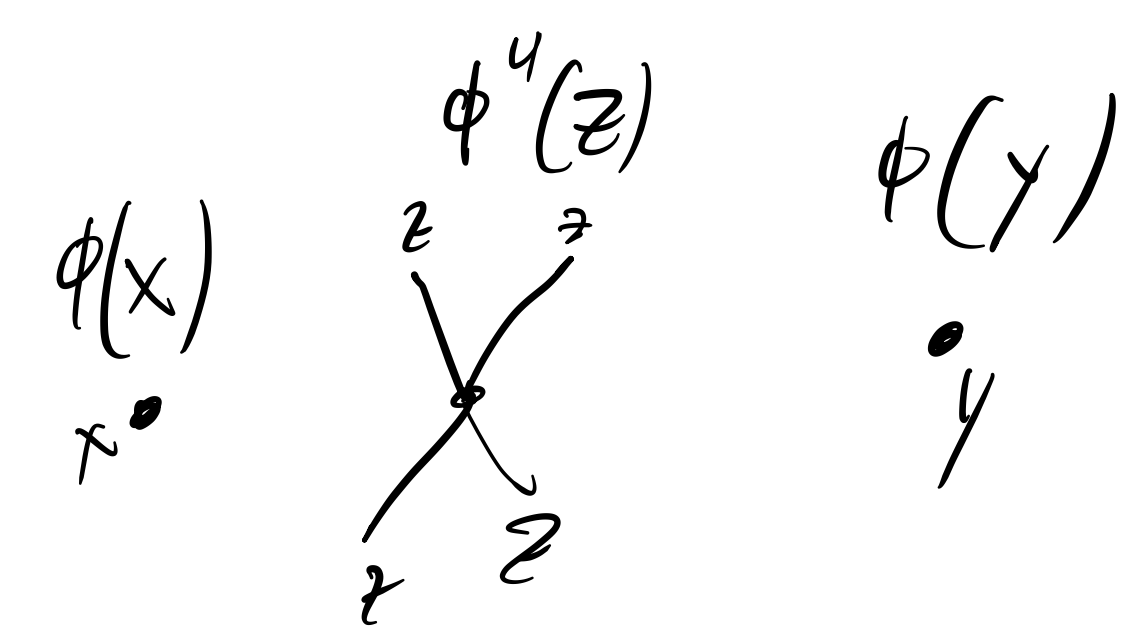
\includegraphics[scale=0.5]{Images/fig-firstordervertices.png}
\end{center}

First, lets think about the $\varphi(x)\varphi(y)\varphi^4(z)$ term.

The simplest possible pairing would be pairing $\varphi(x)$ and $\varphi(y)$, and then the $\varphi^4(z)$ to itself. There are 3 possible ways to pair the legs of the $\varphi^4(z)$ term. We then obtain from Wick's theorem:
\begin{equation}
   -i\frac{3\lambda}{4!}\int dz \Delta^2(z, z)\Delta(x, y).
\end{equation}

\begin{center}
   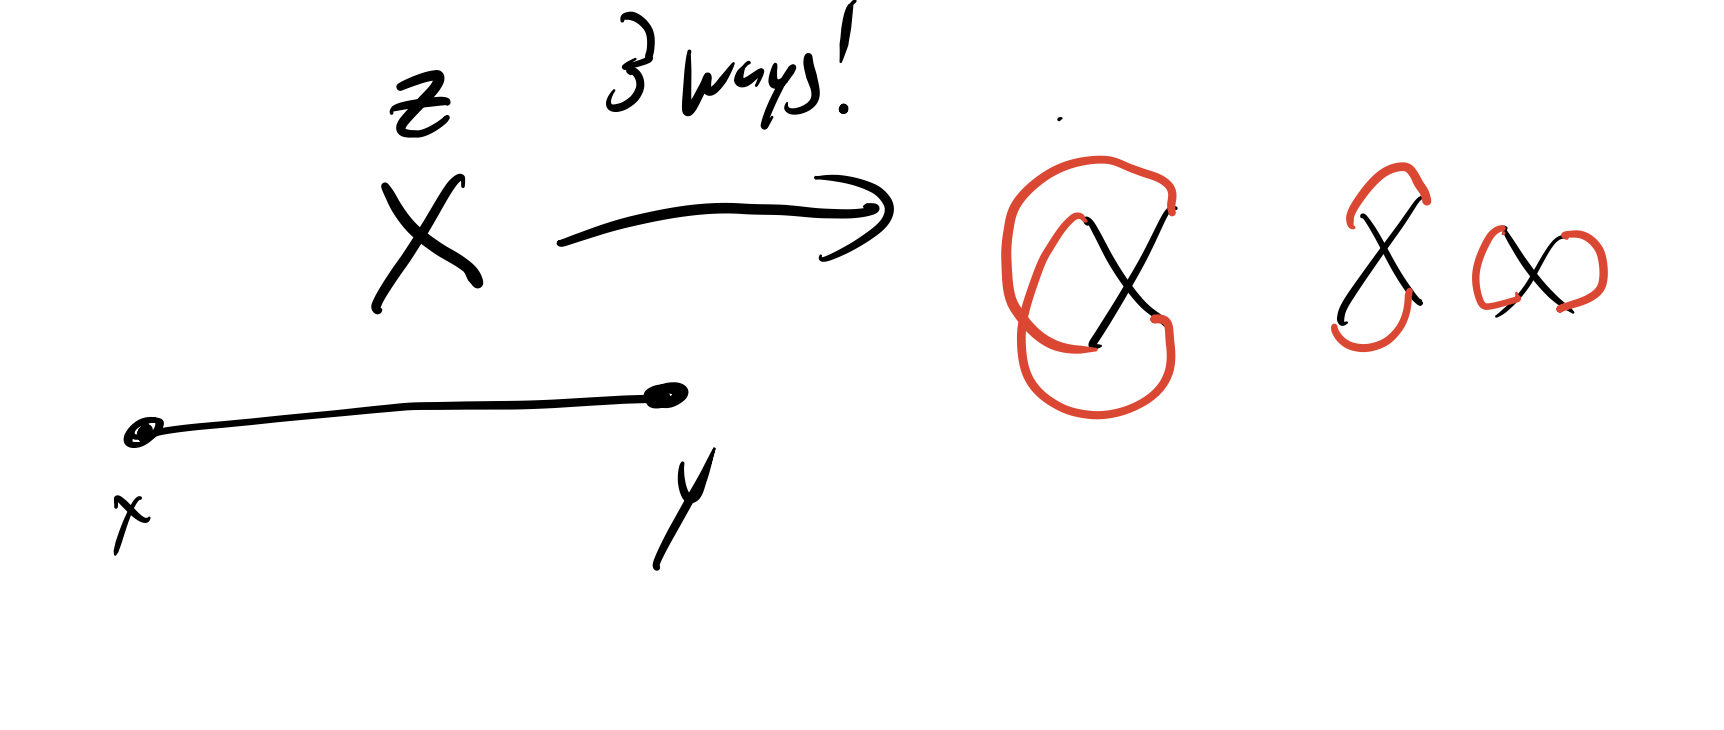
\includegraphics[scale=0.5]{Images/fig-firstorderpairing1.png}
\end{center}

All of the other possibilities have the $\varphi(x)$ and $\varphi(y)$ pairing with the $\varphi^4(z)$. There are four legs to choose from for $x$, then three remaining legs to choose from for $y$, and then the remaining two legs pair with itself, so we have $4 \cdot 3 \cdot 1 = 12$ choices and so:
\begin{equation}
   -i\frac{4 \cdot 3}{4!}\lambda \int dz \Delta(z, z)\Delta(x, z)\Delta(z, y)
\end{equation}

\begin{center}
   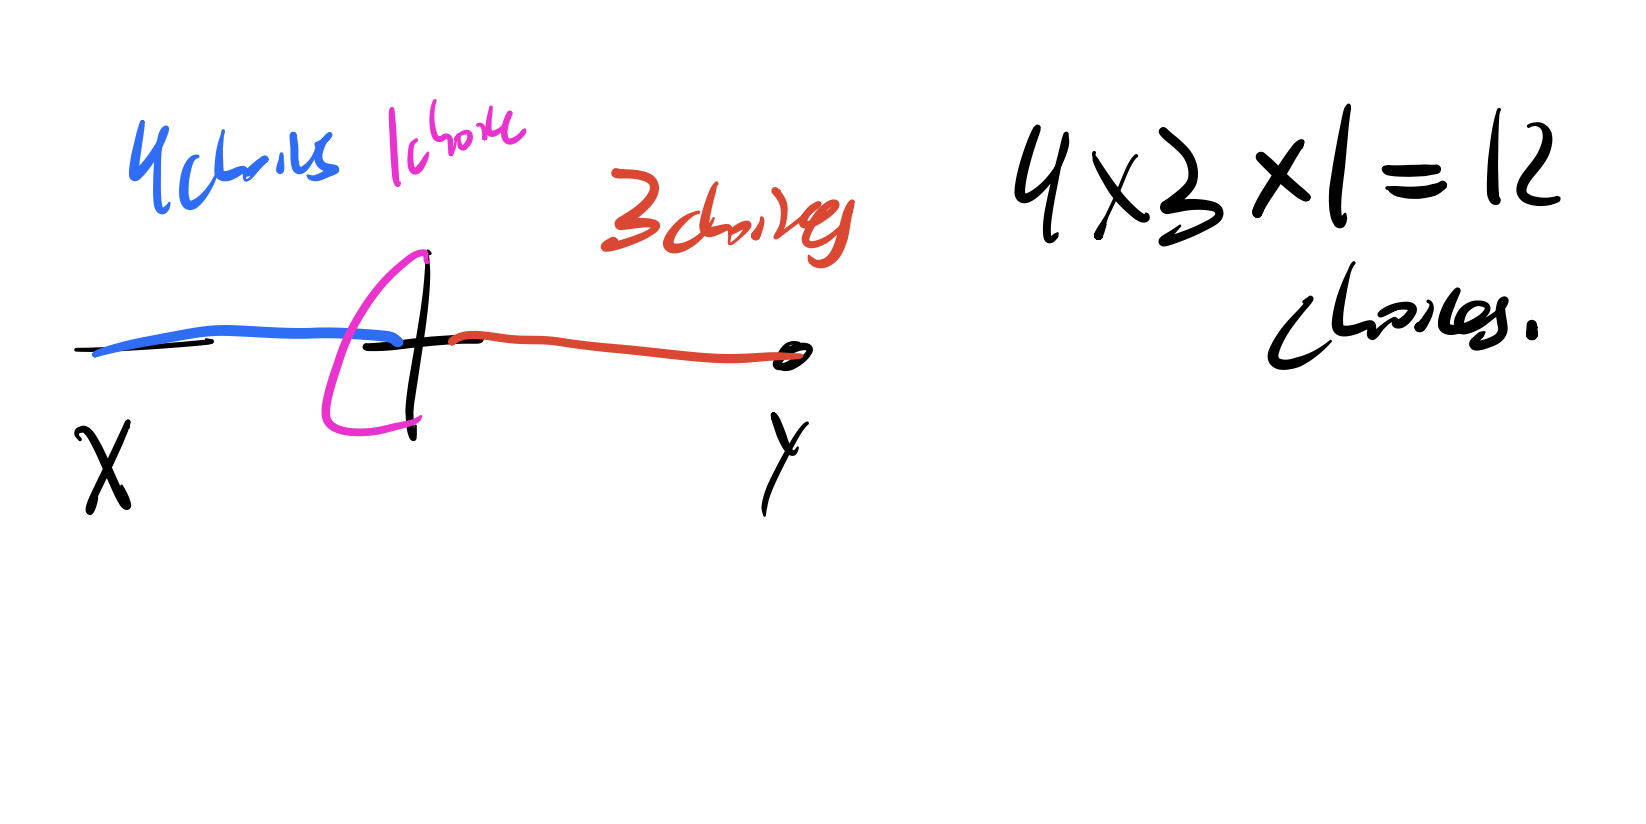
\includegraphics[scale=0.5]{Images/fig-firstorderpairing2.png}
\end{center}

That's it for the pairings! Then we worry about the counterterms, i.e. the terms:

\begin{equation}
   \varphi(x)\varphi(y)\left(\frac{\lambda m}{2}z^{(1)}_m \varphi^2(z) + \frac{\lambda z^{(1)}}{2}\p_\mu \varphi(z)\p^\mu \varphi(z)\right)
\end{equation}

For the first thing we have just a line, one pairing between $\varphi(z), \varphi(z)$ so:
\begin{equation}
   -\frac{i\lambda}{2}\int dz(-z^{(1)} \p^2 \Delta(z, z) - m^2z_m^{(1)}\Delta(z, z))
\end{equation}

\begin{center}
   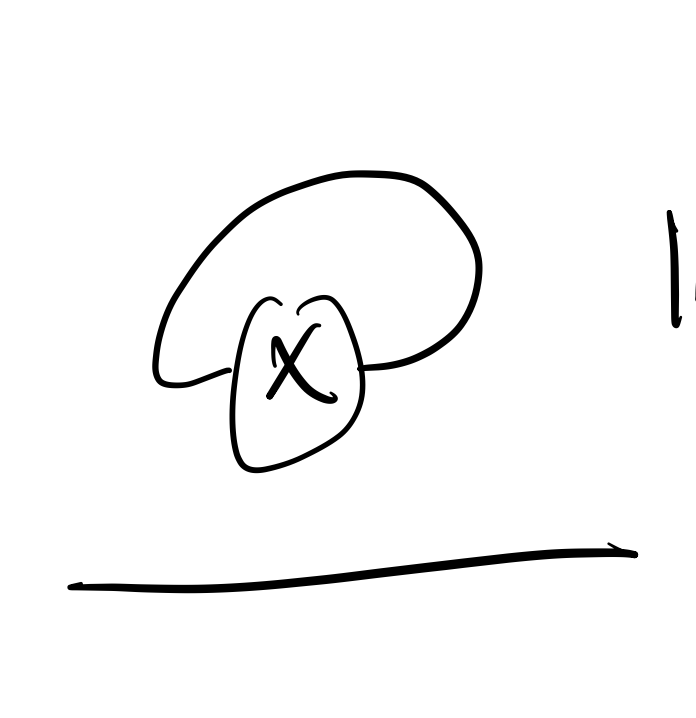
\includegraphics[scale=0.5]{Images/fig-firstordercounterterm1.png}
\end{center}

For the next, we have two pairings between $\varphi(z), \varphi(x)$ and $\varphi(z), \varphi(y)$ and so:
\begin{equation}
   -i\lambda \int dz \Delta(x, z)(-z^{(1)}\p^2 + m^2 z^{(1)}_m)\Delta(z, y)
\end{equation}

\begin{center}
   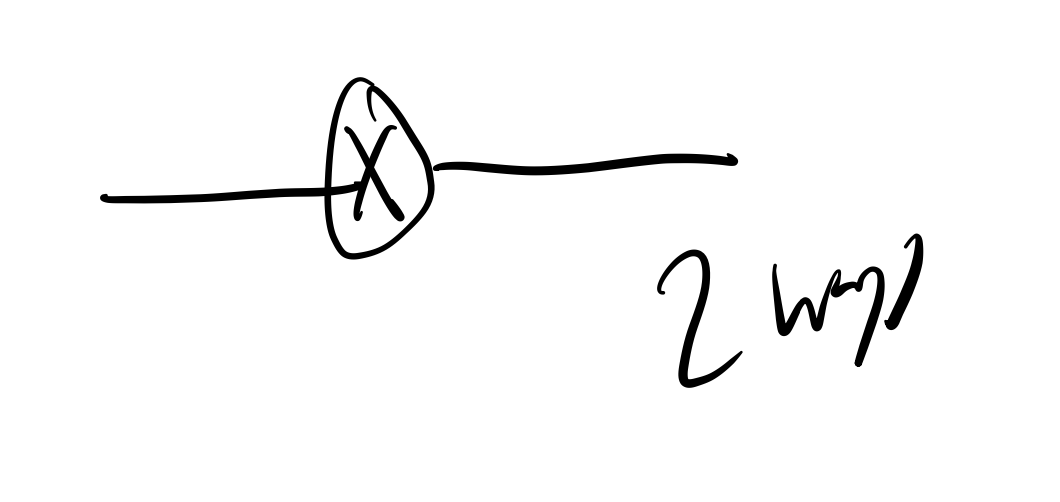
\includegraphics[scale=0.5]{Images/fig-firstordercounterterm2.png}
\end{center}


Now, let's worry about the third term in our expansion of $D(x, y)$. What will happen is when we look at the pairings, it will be the sum of:

\begin{center}
   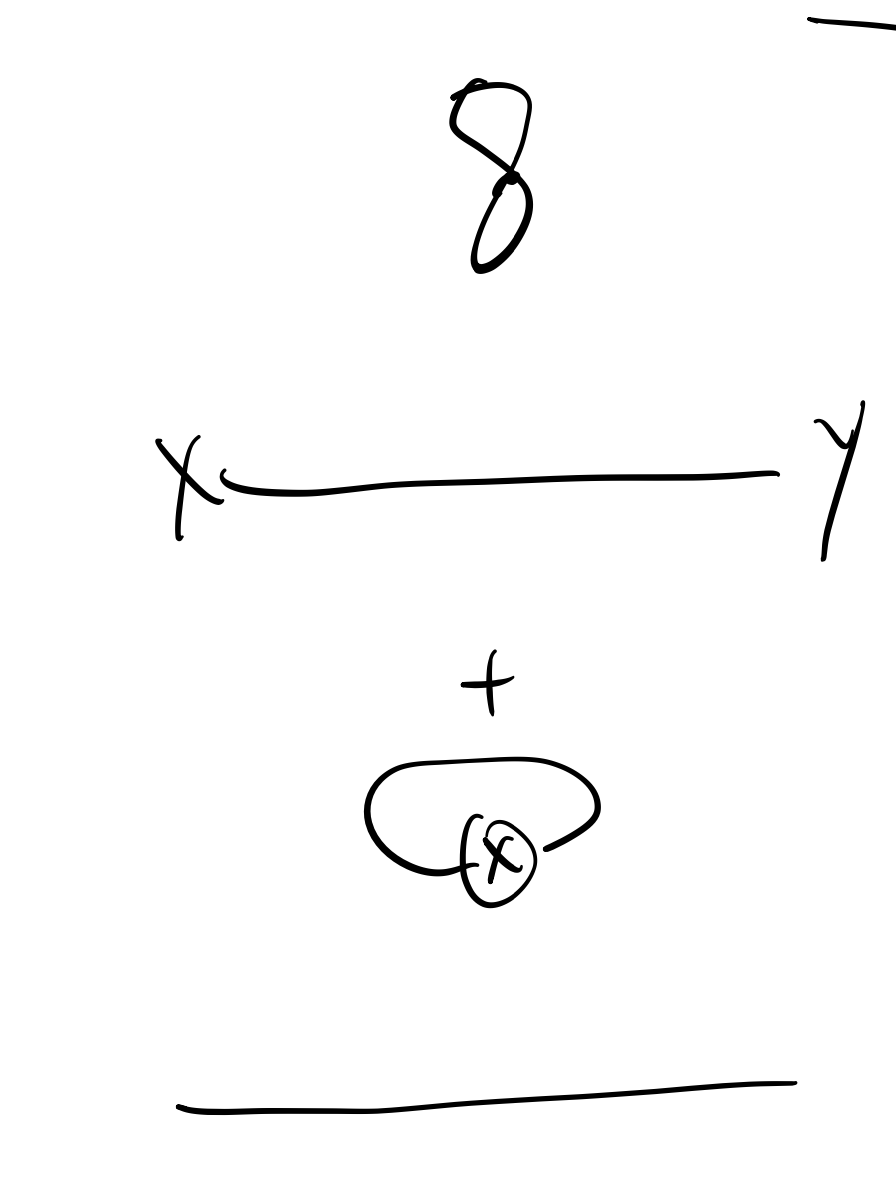
\includegraphics[scale=0.5]{Images/fig-firstordercancellations.png}
\end{center}


And this will actually cancel out the terms in the first term! We can prove that this always happens, using functional integral techniques. This is known as Goldstone's theorem. Anyone who calculates Feynman diagrams should really take their hats off to him because it saves us a lot of time!

Why those two? Each of the two that are removed have a subdiagram that is connected to external legs. This is known as a vacuum bubble. Goldstone's theorem tells us we may ignore such vacuum bubble terms.

Now the punchline: 
\begin{equation}
   D(x, y) = \Delta(x, y) - i\frac{\lambda}{2}\int d^4z \Delta(x, z)\Delta(z, z)\Delta(z y) - i\lambda \int d^4z \Delta(x, z)(-z^{(1)}\p^2 + m^2 z^{(1)}_m)\Delta(z, y) + O(\lambda^2)
\end{equation}
So our final result is quite short! At this point, we could choose parameters such that we are as close to free field theory as we could get. We could choose the $m^2 z^{(1)}_m$ to cancel out $\Delta(z, z)$ and the $z^{(1)}$ to be zero as we have no other derivative terms. And this would be a wise choice - this would keep $m^2$ to the actual mass, and give a nice normalization for $\varphi$. At this point we will stop.

A comment - this is not a convergent series (this can be seen because the series has a radius of convergence of zero, as it diverges for when $\lambda < 0$); it is an asymptotic expansion. We can go up to a certain order and stop when it starts to blowup. For QED its about 50 orders in $\alpha$, for QCD its only a few orders (note the coupling constant is $\sim \frac{1}{3}$ so strong interactions are hard!)

Next time we make this more sophisticated.